%%%% Paramétrage du TD %%%%
\def\xxactivite{Colle 03 \ifprof -- Corrigé \else \fi} % \normalsize \vspace{-.4cm}
\def\xxauteur{\textsl{Xavier Pessoles}}


\def\xxnumchapitre{Chapitre 1 \vspace{.2cm}}
\def\xxchapitre{\hspace{.12cm} Correction des systèmes}

\def\xxcompetences{%
\textsl{%
\textbf{Savoirs et compétences :}\\ \vspace{-.4cm}
\begin{itemize}[label=\ding{112},font=\color{ocre}]
\item \textit{C1-02 : }Proposer une démarche de réglage d'un correcteur.
\item \textit{C2-04 : }Mettre en œuvre une démarche de réglage d’un correcteur.
\end{itemize}
}}

\def\xxtitreexo{Réglage d'un correcteur proportionnel et d'un correcteur à avance de phase}
\def\xxsourceexo{\hspace{.2cm} Equipe PT -- La Martinière Monplaisir}
\def\xxauteur{\textsl{Xavier Pessoles}}

\def\xxfigures{
%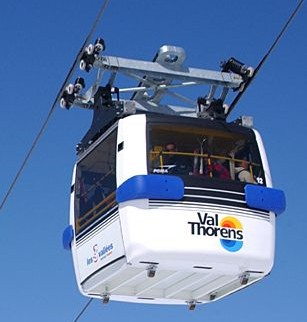
\includegraphics[width=.35\linewidth]{fig_00}
}%figues de la page de garde


\input{\repRel/Style/pagegarde_TD}
\setcounter{numques}{0}


\setlength{\columnseprule}{.1pt}

\pagestyle{fancy}
\thispagestyle{plain}

\vspace{4.9cm}

\def\columnseprulecolor{\color{ocre}}
\setlength{\columnseprule}{0.4pt} 

%%%%%%%%%%%%%%%%%%%%%%%

\setcounter{exo}{0}
\begin{multicols}{2}

%\section*{}

On considère un système de fonction de transfert est :  $G(p)=\dfrac{K}{(p+1)^3}$ placé dans une boucle de régulation à retour unitaire. On souhaite une marge de phase supérieure à 45\degres.

\question{Définir la condition de stabilité théorique du système ? }


On note $t_m$ le temps de montée du système en BF avec  $t_m\simeq \dfrac{3}{\omega_{\text{co}}}$ et $\omega_{\text{co}}$ est la pulsation de coupure à \SI{0}{dB} du système en BO.  


\question{Calculer la valeur $K$ qui assure, en boucle fermée, un temps de montée de \SI{2,15}{s}.}

\question{Calculer pour cette valeur de $K$ la marge de phase.}

\question{En déduire l'expression de la fonction de transfert du correcteur à avance de phase $C(p)=K_a\dfrac{1+aTp}{1+Tp}$ qu'il faut introduire dans la chaîne directe.  }

\end{multicols}
\ifprof
\newpage
\begin{center}

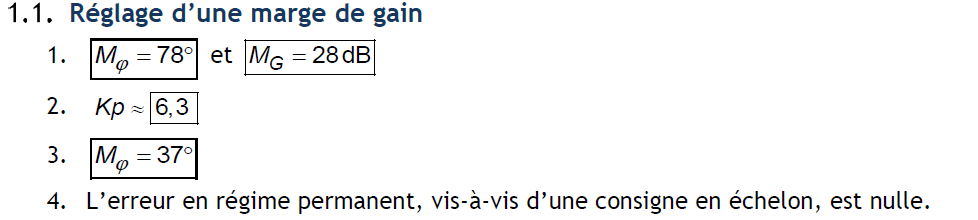
\includegraphics[width=\linewidth]{cor_01}
\end{center}
\else
\fi
